
\documentclass{article}
\usepackage{graphicx}
\usepackage[top=3cm]{geometry}
\usepackage{tabularray}
\usepackage{afterpage}
\usepackage{amsmath}
\usepackage{listings}
\usepackage{subcaption}
\usepackage{mwe}
\lstset{language=Matlab}

\graphicspath{{./}}
\begin{document}

\begin{titlepage}
	\begin{center}
	\LARGE{ECE 8540 Analysis of Tracking System}\\
	\line(1,0){200}\\
	[5mm]
	\Large{Lab 3 report}\\
	\Large{Model Fitting}\\
	[150mm]
	\large{Harshal B. Varpe}\\
	September 27, 2022
	\end{center}
\end{titlepage}

\begin{center}
\section{Introduction}\label{sec:intro}
\end{center}
Lab 1 focuses on calculating a linear regression fit for the given data sets. Linear regression is used to obtain the values of one variable with respect to another variable. Student were to construct appropriate matrices using normal equations to determine the unknowns and then plot the results. Normal equations are equations obtained by setting the partial derivatives of the sum of squared errors to zero. For the first two parts, data set contained five data points, whereas for the third part we had large amount of scattered data points.
The general line fitting equation is given by - 
\begin{equation}\label{eqn1}
y = a_1f_1(x)+a_2f_2(x)+...+a_Mf_M(x)
\end{equation}
where $a_1,..,a_M$ are the M number of linear unknowns. The terms $f_1(x),f_2(x),..,f_M(x)$ are called basis functions. Unlike the unknowns, the basis functions need not be linear. Due to the linear nature of the unknowns, these problems are known as linear model fitting or regression problems. The solution to the general line fitting equation is obtained by solving the normal equations. In the next section, we will take a look into the derivation of narmal equations and how to solve them in matlab.

\bigbreak


\section{\centering Methods}\label{sec:meth}


Let us take an example of a straight line. The generalised equation of a line has form - 
\begin{equation}\label{eqn2}
y = mx + c = a_1f_1(x)+a_2f_2(x)
\end{equation}
 Here, $m$ and $c$ are constants and unknowns. $m$ and $c$ are slope and y-intercept of the line respectively. \\
For a given set of data points $(x_i,y_i) \forall i = 1,...,N $ , we define the residual $e_i$ for each $ (x,y) $ as follows -
\begin{equation}\label{eqn3}
e_i = y_i - \sum_{i=1}^{M} (a_if_i(x_i))
\end{equation}

Chi-squared error metric is difference between the best fitting solution and the collective set of data:
\begin{equation}\label{eqn4}
{\chi}^2(a_1,a_2,...,a_M) = \sum_{i=1}^N \left(y_i - \sum_{j=1}^M(a_if_i(x_i))\right)^2
\end{equation}

The best possible values for the unknowns $a_1,a_2,..,a_M$ are found by taking the partial derivative of ${\chi}^2$ with respect to each of the M unknowns and setting them equal to zero.
The simplified version of this process is as follows :
\begin{equation}\label{eqn5}
\forall k = 1,..,M \sum_{i=1}^N f_k(x_i)y_i = \sum_{i=1}^N\sum_{j=1}^Mf_k(x_i)f_j(x_i)a_j
\end{equation}

We convert the equation \ref{eqn5} into matrix notation to simplify equations.\\
\begin{equation}\label{eqn6}
A = 
\begin{bmatrix}
f_1(x_1) & f_2(x_1) & ... & f_M(x_1) \\
f_1(x_2) & f_2(x_2) & ... & f_M(x_2) \\
. & . & ... & . \\
. & . & ... & . \\
f_1(x_N) & f_2(x_N) & ... & f_M(x_N) \\
\end{bmatrix}
\end{equation}

\begin{equation}\label{eqn7}
x = 
\begin{bmatrix}
a_1 \\a_2 \\. \\. \\a_M \\
\end{bmatrix}
\end{equation}

\begin{equation}\label{eqn8}
b = 
\begin{bmatrix}
y_1 \\y_2 \\. \\. \\y_M \\
\end{bmatrix}
\end{equation}

Equation \ref{eqn5} can be written in matrix form as - 
\begin{equation}\label{eqn9}
A^Tb = A^TAx
\end{equation}

Upon simplifying the equation 9, we can obtain the following form - 
\begin{equation}\label{eqn10}
x = (A^TA)^{-1}A^Tb
\end{equation}

Equation \ref{eqn10} is called the solution to the normal equations. Properly constructed matrices $A,x, $and $b$ can be used to solve any problem in the form of equation \ref{eqn1}.

For the part 1 of the problem, the data set is as follows - $(5,1),(6,1),(7,2),(8,3),(9,5)$

Therefore, the $A,x, $and $b$ matrices can be written as - 

\begin{equation}\label{eqn11}
A = 
\begin{bmatrix}
 5&1\\6&1\\7&1\\8&1\\9&1
\end{bmatrix}
\end{equation}

\begin{equation}\label{eqn12}
x = 
\begin{bmatrix}
m (slope) \\ b (y-intercept)
\end{bmatrix}
\end{equation}

\begin{equation}\label{eqn13}
b = 
\begin{bmatrix}
1\\1\\2\\3\\5
\end{bmatrix}
\end{equation}
 The following code snippet shows the MATLAB code for solving problem 1.\\
\begin{lstlisting}[frame=single]
% Part 1 %

c = [5,6,7,8,9];
d = [1,1,2,3,5];

A = [c' ones(5,1)];
b = [d'];
x = inv(A'*A)*A'*b
% Here first element of x is a and second element is b.%
% y = ax + b%
i = 0:0.1:10;
y = x(1)*i + x(2);
plot(c,d,"ko",i,y,"k")
xlabel("X-axis")
ylabel("Y-axis")
txt = {'First Line:','y = 1.000x-4.600'}
text(8,2,txt)
% ylim([0 6])
% legend("Data Points","Fitted Line","Location","best")
% hold on

\end{lstlisting}

In the part 2 of the problem, we are given an additional point in addition to the data points given for part 1. Hence, the dataset for part is:
$(5,1),(6,1),(7,2),(8,3),(9,5),(8,14) $
We can construct the $A,x, $and $b$ matrices thusly -

\begin{equation}\label{eqn14}
A = 
\begin{bmatrix}
 5&1\\6&1\\7&1\\8&1\\8&1\\9&1
\end{bmatrix}
\end{equation}

\begin{equation}\label{eqn15}
x = 
\begin{bmatrix}
m (slope) \\ b (y-intercept)
\end{bmatrix}
\end{equation}

\begin{equation}\label{eqn16}
b = 
\begin{bmatrix}
1\\1\\2\\3\\14\\5
\end{bmatrix}
\end{equation}
 The figure following shows the MATLAB code snippet for solving problem 1.\\
\begin{lstlisting}[frame=single]
% Part 2 

c1 = [5,6,7,8,8,9];
d1 = [1,1,2,3,14,5];

A1 = [c1' ones(6,1)];
b1 = [d1'];
x1 = (inv(A1'*A1)*A1')*b1

y1 = x1(1)*i + x1(2);
plot(c1(5),d1(5),"ro",i,y1,"k") %Plotting only the outlier
ylim([0 15])
xlabel("X-axis")
ylabel("Y-axis")
legend("Data Points","Fitted Line","Outlier","Location","northwest")
txt = {'Second Line:','y = 1.8154x-8.6769'};
text(5,5,txt);
hold off;
\end{lstlisting}
\pagebreak
Part 3 of problem deals with a dataet of 83 people and their 3398 meals. For the purpose of model fitting, we observed the relationship between the number of bites taken by a person and Kilocalories consumed per Bite. In order to fit a model to this data, we first plot the data and observe a general trend. This trend helps in deciding what models would be provide good fit and what model would be ill-suited.\\
\begin{figure}[!htb]
\centering
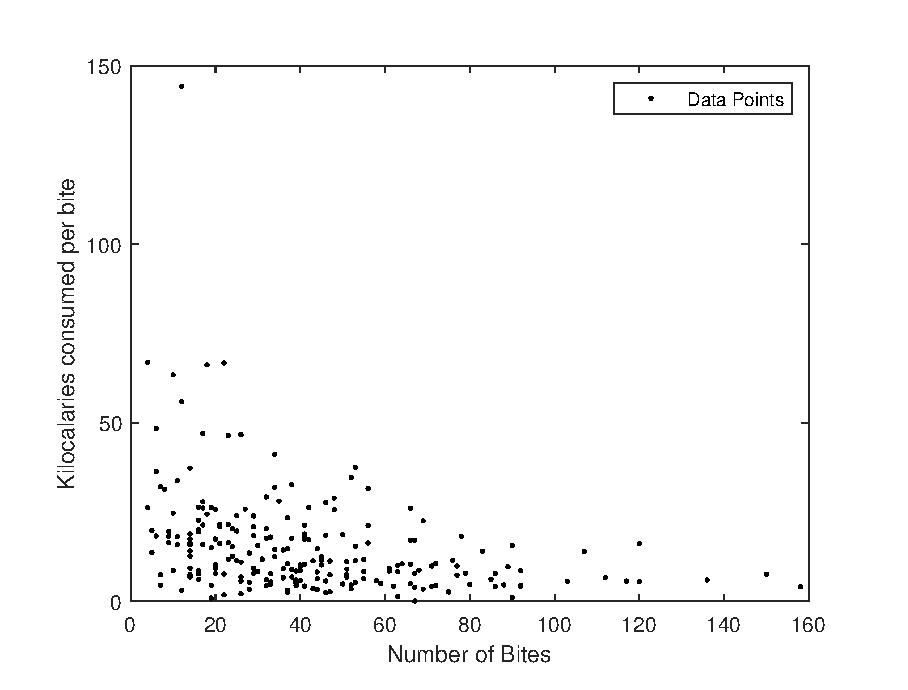
\includegraphics[scale=0.8]{meal_data_15th.eps}
\label{plt:1}
\caption{Plot of the meal data set (\small{every 15th point })}
\end{figure}

\vspace{10mm}
For the plot above, we have selected every 15th point from data set. This was done to minimize the overlapping of points. Moreover, we do not need to view every data point to observe the genral trend in data. From the observation of the plot, we can safely assume that there is an inverse relationship between the numer of bites taken and Kilocalories consumed. It is also worth noting that the nature of this relationship is not linear and fitted curve will probably as asymptotic nature. This is because, it is impossible to consume any amount Kilocalories with zero bites and vice versa. Based on this, a few models were tried on the graphical calculator to observe their suitability.

\begin{figure}[!htb]
     \centering
     \begin{subfigure}[b]{0.4\textwidth}
         \centering
         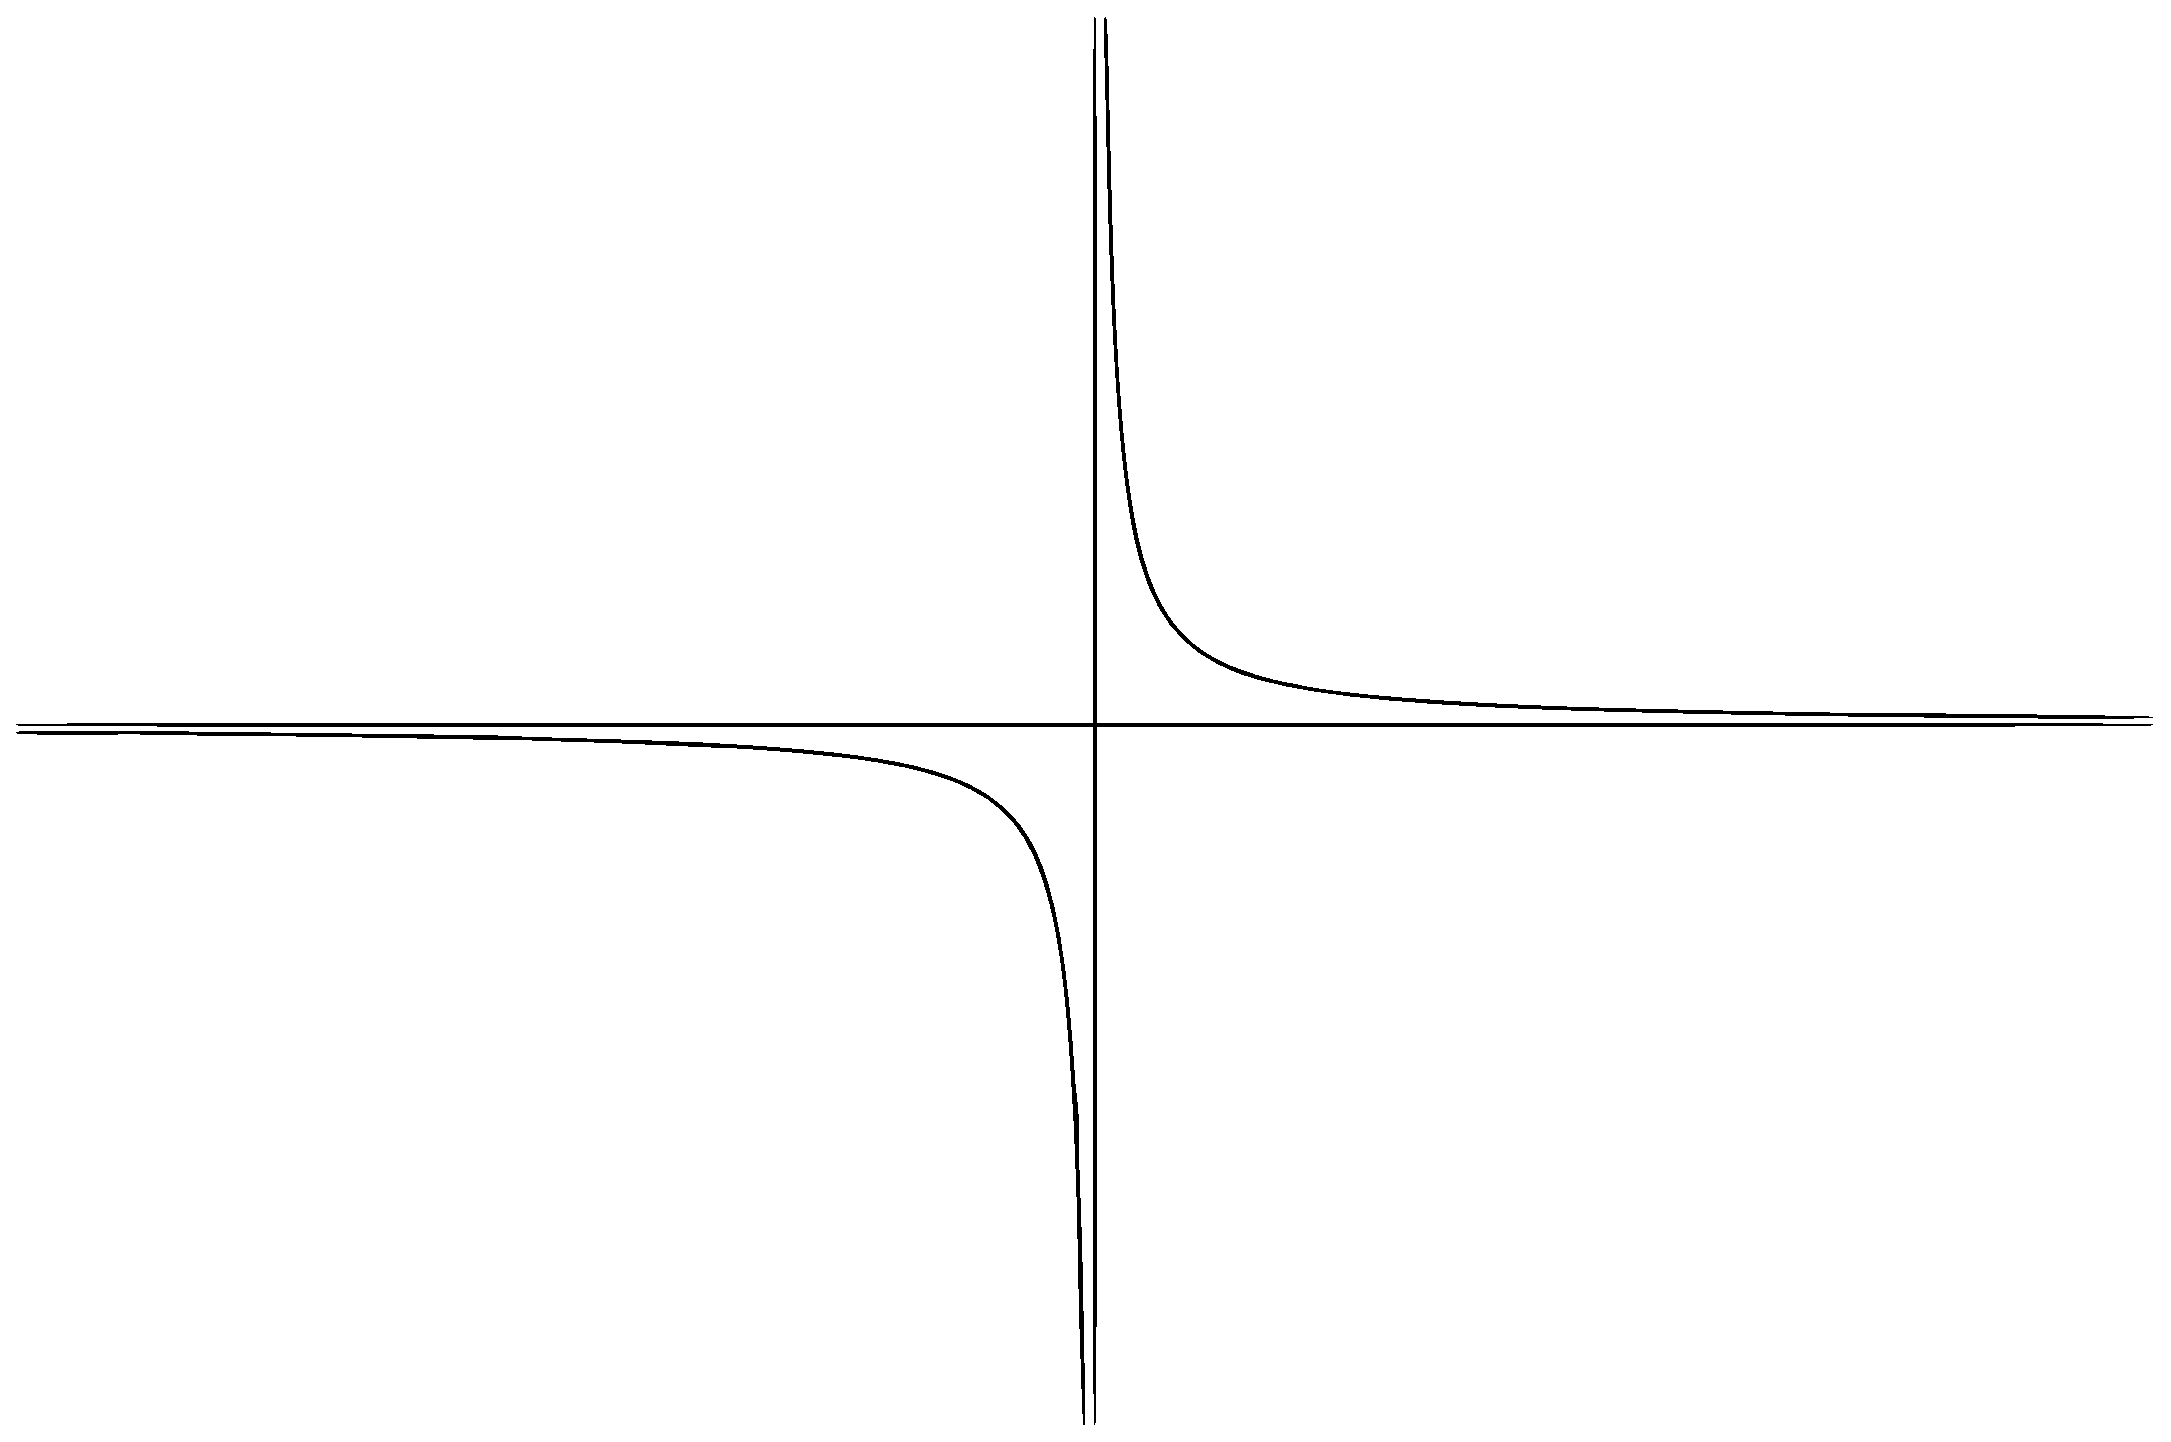
\includegraphics[width=\textwidth]{First_model.eps}
         \caption{$y=a(1/x)+ b $}
         \label{plt:14}
     \end{subfigure}
     \hfill
     \begin{subfigure}[b]{0.5\textwidth}
         \centering
         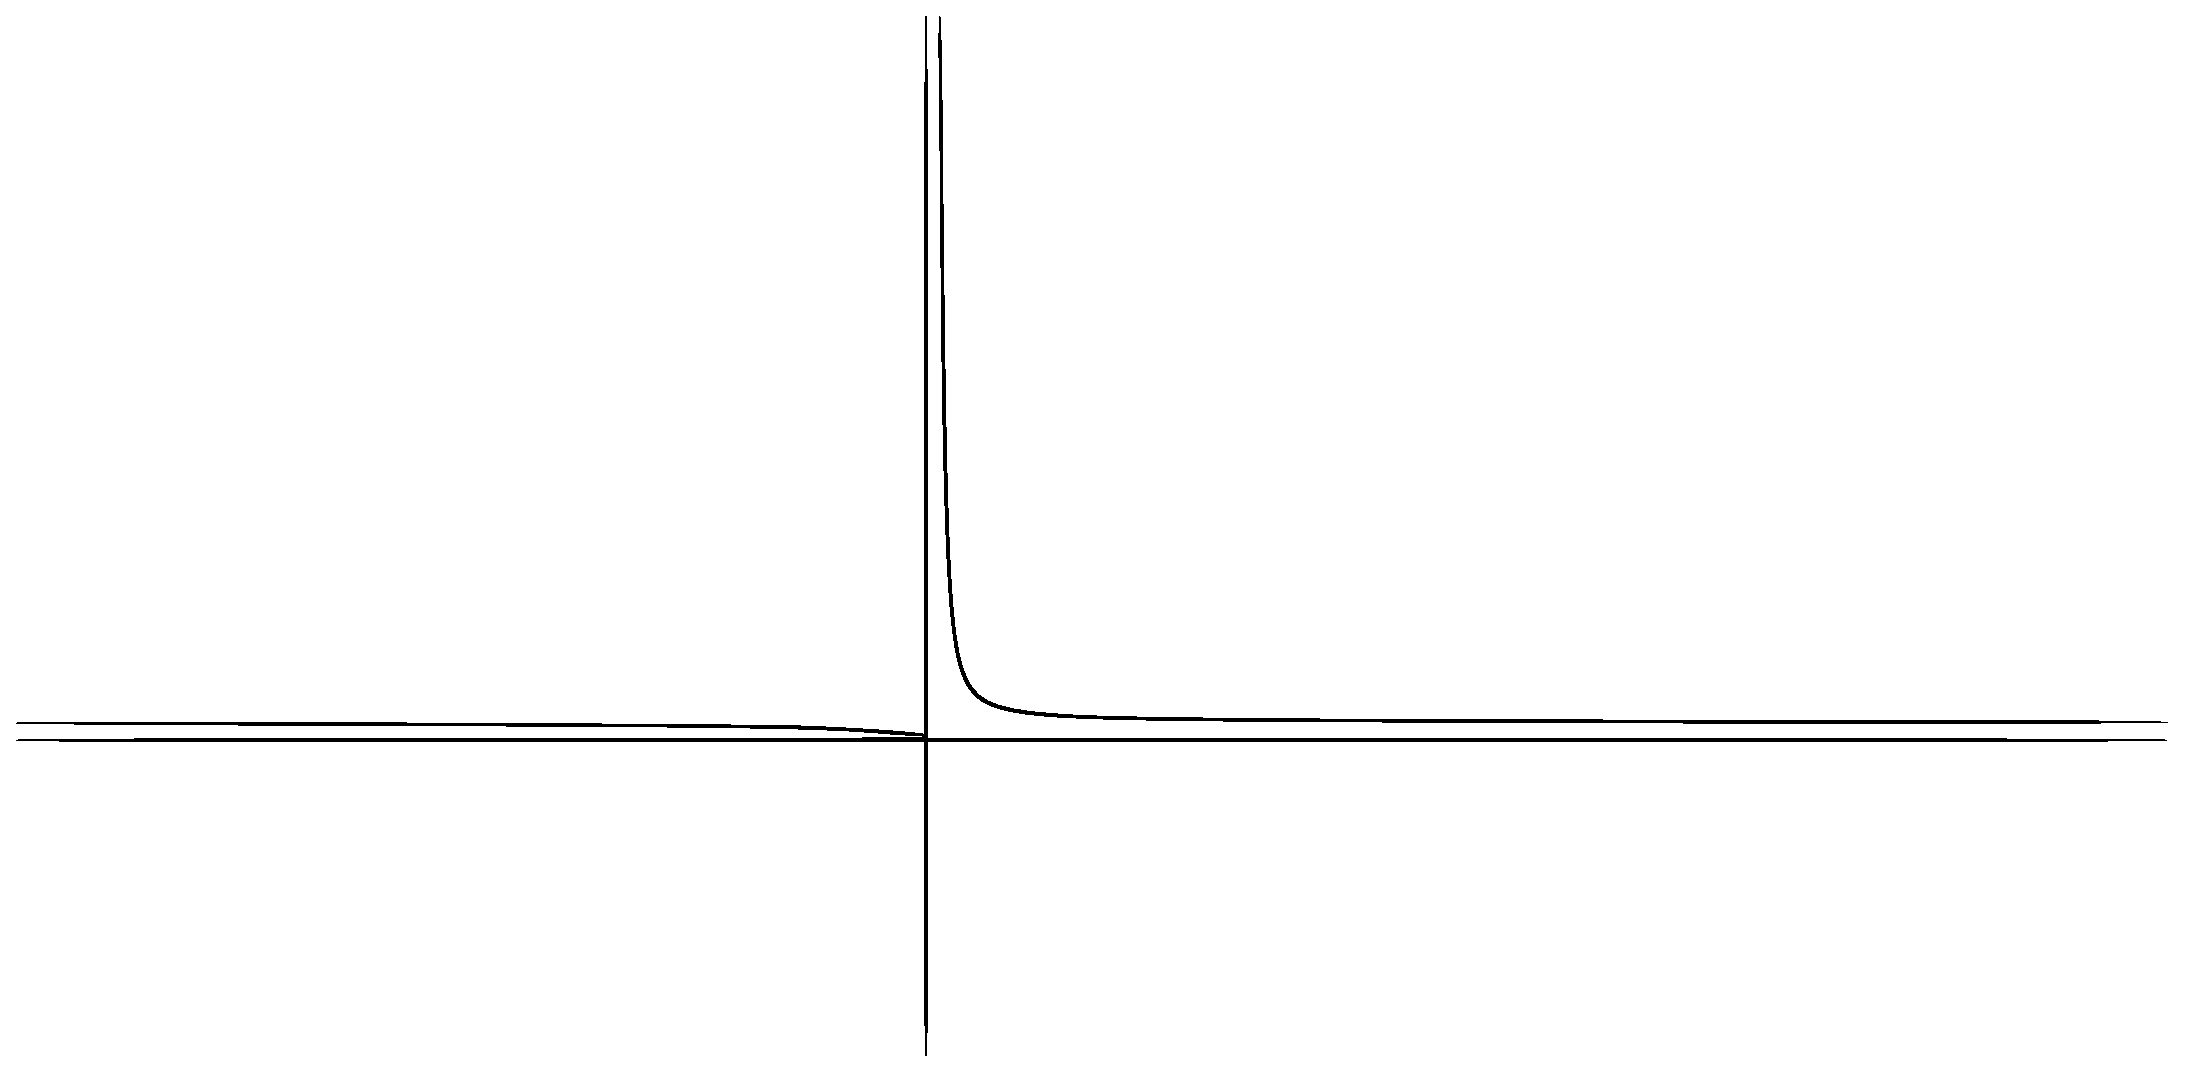
\includegraphics[width=\textwidth]{Second_model.eps}
         \caption{$ y=a*e^{1/x}+ b$}
         \label{plt:24}
     \end{subfigure}
     \vskip\baselineskip
     \begin{subfigure}[b]{0.4\textwidth}
         \centering
         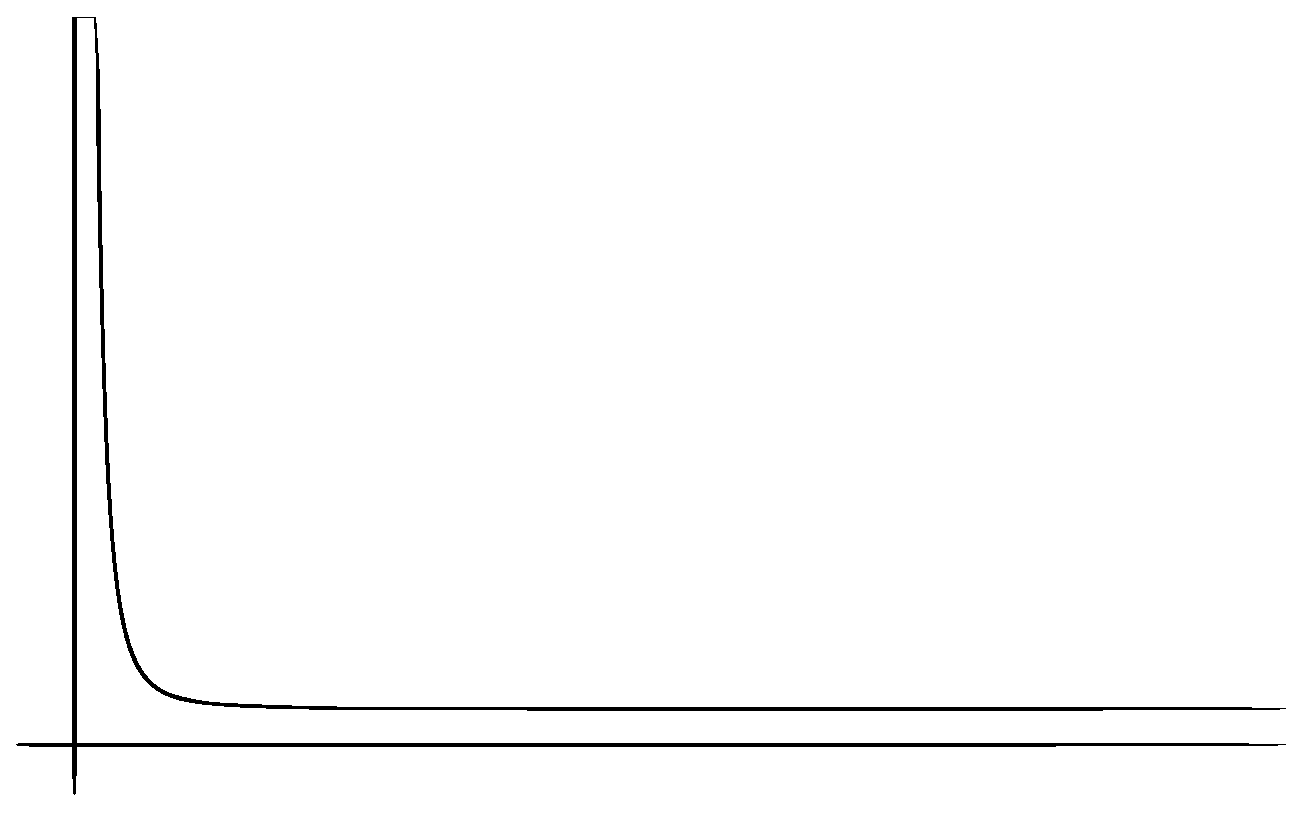
\includegraphics[width=\textwidth]{Thrd_model.eps}
         \caption{$y=a(1/x^{e})+ b$}
         \label{plt:34}
     \end{subfigure}
	\hfill
     \begin{subfigure}[b]{0.4\textwidth}
         \centering
         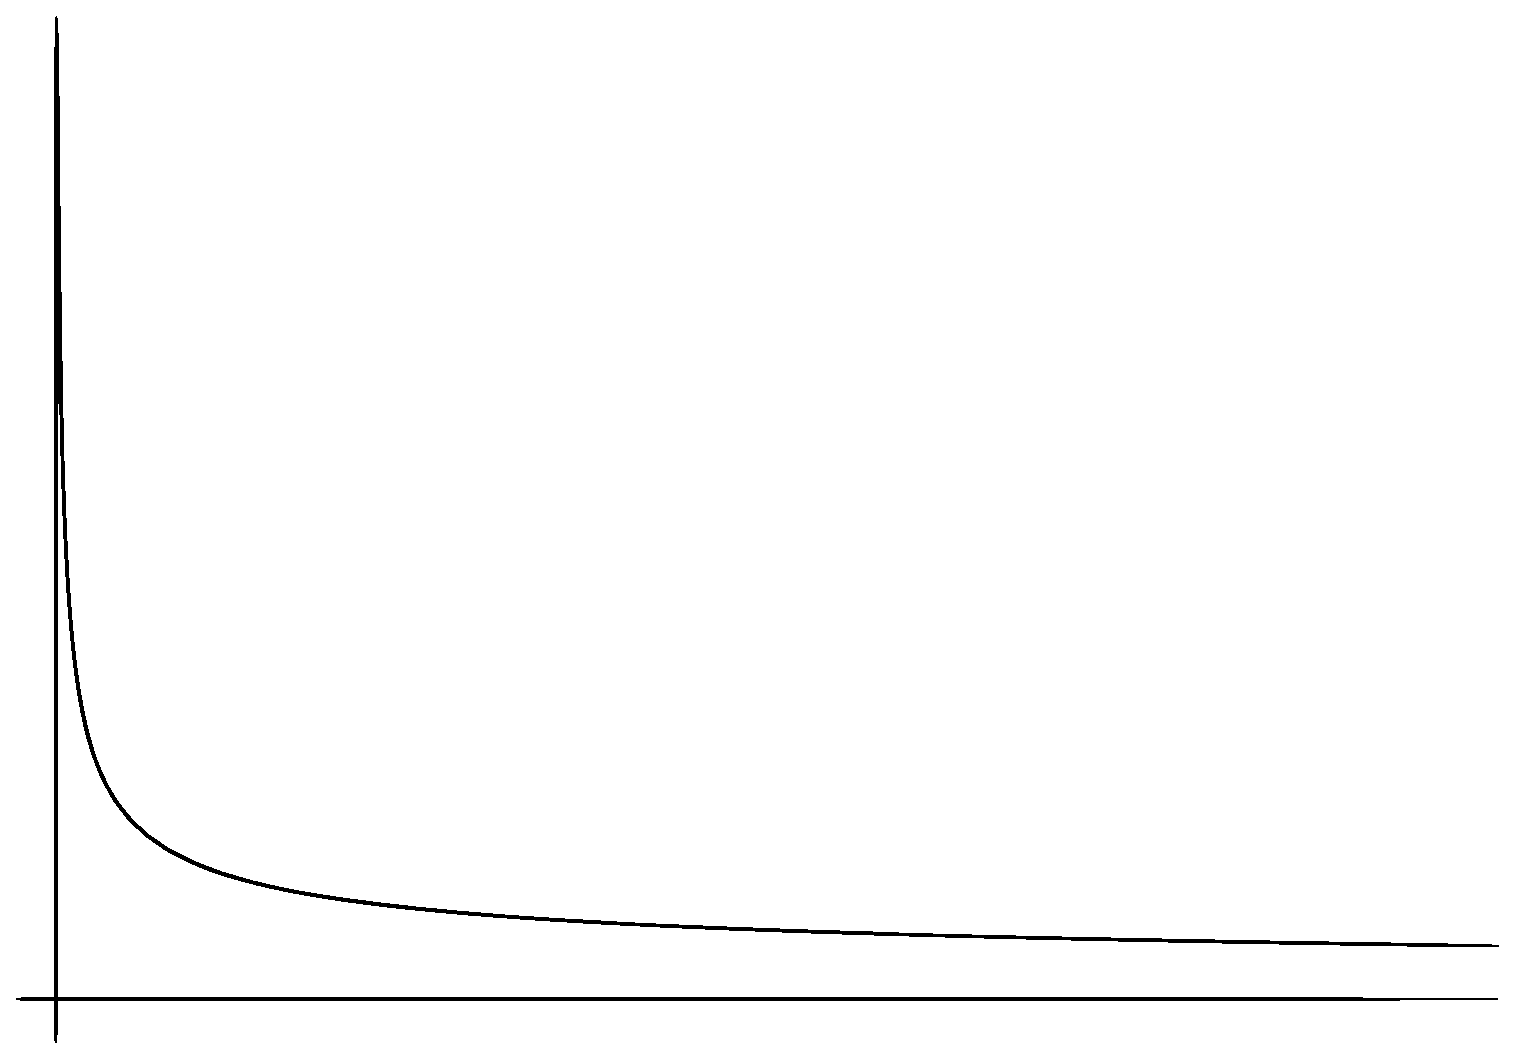
\includegraphics[width=\textwidth]{Fourth_model.eps}
         \caption{$y=a*1/(x^{1/2}) + b$}
         \label{plt:44}
     \end{subfigure}
        \caption{Plots of Different models }
        \label{fig:models}
\end{figure}

\newpage
The first model that was tried was: $y=a(1/x)+ b$
Superficially, it seems that this model would work. However, we have no negative values in our data. Our data lies only in the first quadrant since the given quantities cannot be negative. Clearly, this model is ill-suited. The plot of this function in shown in figure \ref{plt:14}.\\
The second model was : $y=a*e^{1/x}+ b$
We can see from the figure \ref{plt:24}, that this model is more promising than the first one. However, it is still not appropriate for the dataset we have, since it goes into second quadrant for some values of x. This behaviour is unwanted.\\
The third model was : $y=a(1/x^{e})+ b$
This function shows good fit for the data we have. It is certainly better than previous two models, since it lies mostly in the first quadrant.This model was chosen as the first model to solve using normal equations. The plot in figure \ref{plt:34} shows the nature of this function.\\
The fourth model tried for fitting was : $y=a*1/(x^{1/2}) + b$
The plot in figure \ref{plt:44} shows the nature of this function. Model three seems to suggest that for certain lower range of number of bites, Kilocalories consumed are very high and then Kilocalories consumed are constant irrespctive of number of bites taken. Therefore, there was a need to try out another model.

For the function $y=a(1/x^{e})+ b$ , we can construct the normal equation is matrix form as follows:
\begin{equation}
A=
\begin{bmatrix}
\frac{1}{X_1^e}&1\\
\frac{1}{X_2^e}&1\\
.&.\\
.&.\\
.&.\\
\frac{1}{X_N^e}&1\\
\end{bmatrix}
\end{equation}

\begin{equation}
b=
\begin{bmatrix}
y_1\\
y_2\\
.\\
.\\
.\\
y_N\\
\end{bmatrix}
\end{equation}

\begin{equation}
x=
\begin{bmatrix}
a\\b\\
\end{bmatrix}
\end{equation}
The following figure shows the MATLAB code for the above function.\\
\begin{lstlisting}[frame=single]
c2 = pr_data(1:15:end,1); %Number of bites%
d2 = pr_data(1:15:end,2); %Kilocalories per bite%


A2 = [(1./(c2.^exp(1))) ones(length(c2),1)];
b2 = d2;
x2 = (inv(A2'*A2)*A2')*b2;

fn = 1./o.^exp(1);
y2 = x2(1).*fn + x2(2);
plot(c2,d2,"kx",o,y2,"k-","LineWidth",0.75)
xlim([0 200]);
ylim([0 200]);
xlabel("Number of Bites")
ylabel("Kilocalories per Bite")
legend("Data Points","Fitted Line","Location","best")
title("Meal data Model fitting Model 1")
\end{lstlisting}

For the second function : $y=a*1/(x^{1/2}) + b$, we can form the normal equations in matrix form as follows:

\begin{equation}
A=
\begin{bmatrix}
\frac{1}{\sqrt X_1}&1\\
\frac{1}{\sqrt X_2}&1\\
.&.\\
.&.\\
.&.\\
\frac{1}{\sqrt X_N}&1\\
\end{bmatrix}
\end{equation}

\begin{equation}
b=
\begin{bmatrix}
y_1\\
y_2\\
.\\
.\\
.\\
y_N\\
\end{bmatrix}
\end{equation}

\begin{equation}
x=
\begin{bmatrix}
a\\b\\
\end{bmatrix}
\end{equation}
The following figure shows the MATLAB code for the above function.\\
\begin{lstlisting}[frame=single]
A3 = [(1./sqrt(c2)) ones(length(c2),1)];
b3 = d2 ; %Kilocalories per bite%;
x3 = (inv(A3'*A3)*A3')*b3;
o1 = 0:0.1:500;
fn = 1./sqrt(o1);
y3 = x3(1).*fn + x3(2);
plot(c2,d2,"kx",o1,y3,"k-","LineWidth",0.75)

xlim([0 200]);
ylim([0 200]);
xlabel("Number of Bites")
ylabel("Kilocalories per Bite")
legend("Data Points","Fitted Line","Location","best")
title("Meal data Model fitting Model 2")
\end{lstlisting}


\newpage
\section{\centering Result}\label{sec:code}
For the part 1 of the problem, after solving the normal equations, we get the values of the unknowns i.e. Slope and the y-intercept. Thus the matrix x becomes:
\begin{equation}
x=
\begin{bmatrix}
1\\-4.6
\end{bmatrix}
\end{equation}
We put these values back in equation \ref{eqn2} and plot.\\
\begin{figure}[!htb]
\centering
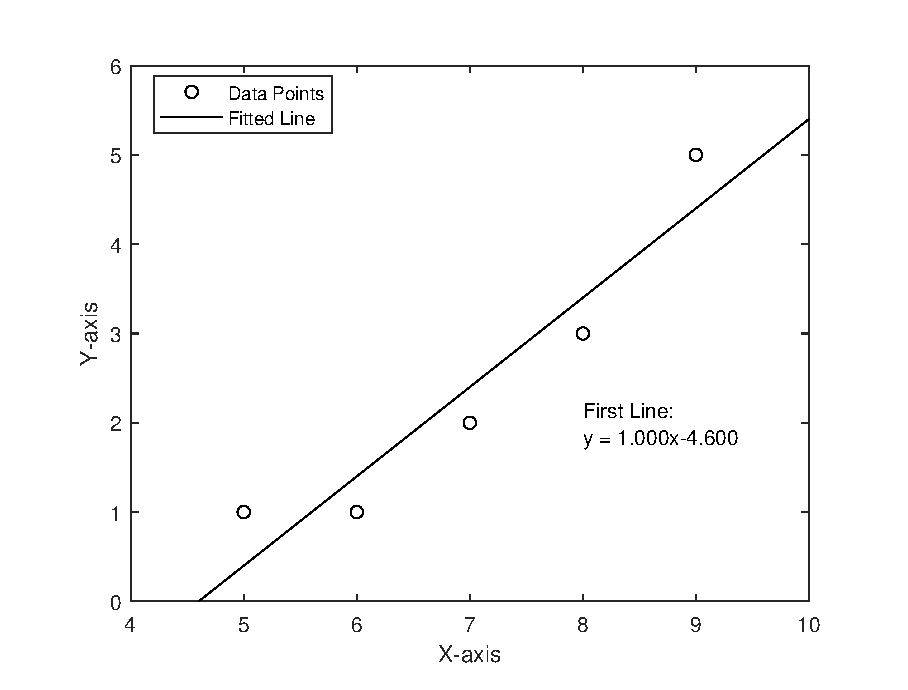
\includegraphics[scale=0.75]{part1.eps}
\caption{Model Fitting Part 1}
\label{fig:part1}
\end{figure}
 The line thus fitted is the line where residual e is minimum for each data point.//
For the part 2 of the problem, we had an additional data point in addition to the data points in part 1. Depending on where this data point lies with respect to the other data points, the nature of curve fitted will change.
After solving the normal equations for the part 2, we get x matrix as follows:

\begin{equation}
x=
\begin{bmatrix}
1.82\\-8.68
\end{bmatrix}
\end{equation}
If we compare the x matrix from part 1 with x matrix obtained in part 2, we notice that with addition of new data point the slop of the fitted line increased as expected. In terms of model fitting, the newly added point negatively affects the model. In other words, we can also say that with addition of second point, the residual increases for the each point in data-set and the model becomes somewhat ill-suited.
The reason for this is that the new point is an outlier.This additional point lies outside of the other values in given dataset. Due to the fact, that new point shows lasrge disparity in y direction with respect to other data points, the slope of the line increases. The increases in slope consequently lowers the y-intercept.

The plot below shows how the outlier affects the curve fitting model adversely. First line refers to the curve obtained for the part 1 of the problem and Second line refers to the curve obtained for part 2 of the problem.\\
\begin{figure}[!htb]
\centering
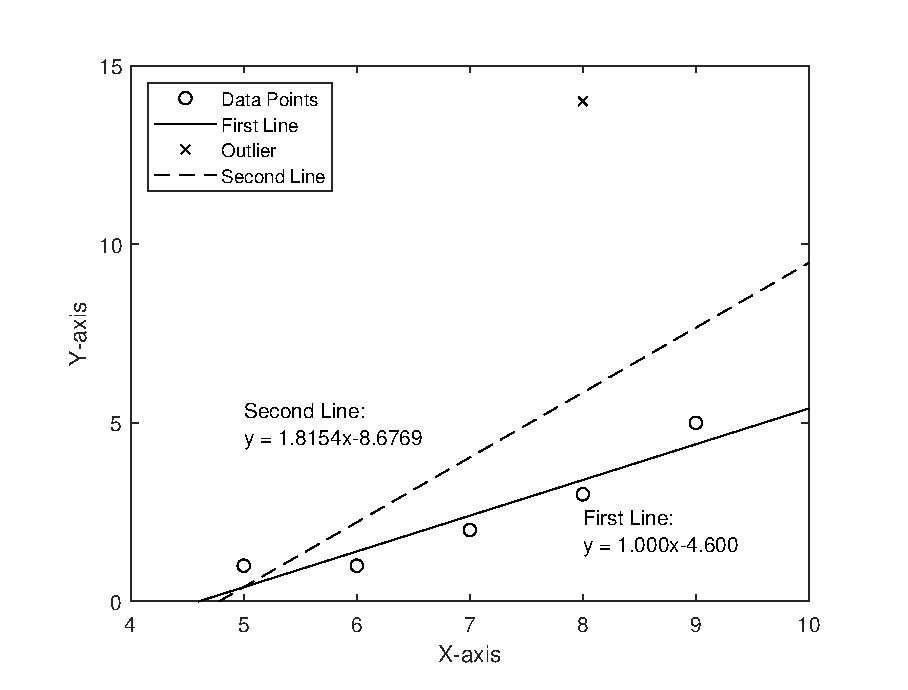
\includegraphics[scale=0.75]{part2.eps}
\caption{Model Fitting Comparison between part 1 and part 2}
\label{fig:part2}
\end{figure}

For the third part of the problem, as mentioned in section \ref{sec:meth}, we had two main functions. For the function $y=a(1/x^{e})+ b$, after solving the normal equations, we get 90.46 and 15.97 as values for $a$ and $b$ respectively. We use these values to fit a cuve through given data points. The figure following shows the curve fitted through the given data with function $y=a(1/x^{e})+ b$.\\
\begin{figure}[!htb]
\centering
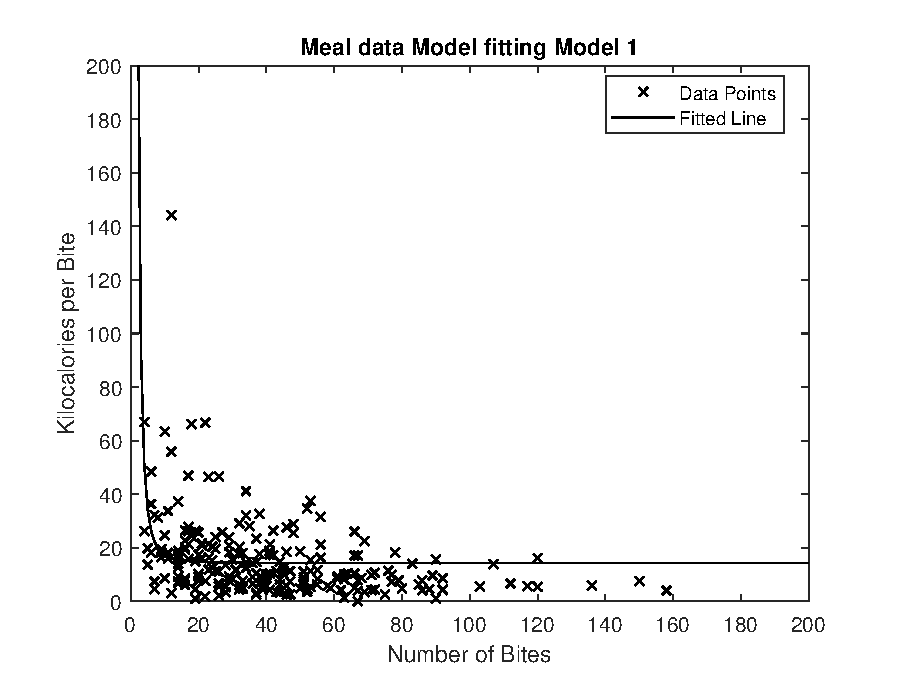
\includegraphics[scale=0.75]{thrd_result.eps}
\caption{Fitted Curve throught meal data for function $y=a(1/x^{e})+ b$ }
\label{fig:thrd_res}
\end{figure}
From the plot we can see, that this model does pretty good job at predicting the relationship between number of bites and Kilocalories consumed per bite, only when the number of bite count is more than 10. This is because the plot seems to suggest, for number of bites is lower than 15, infinite Kilocalories can be consumed. This is impossible.\\

\par
For the function $y=a*1/(x^{1/2}) + b$, we get the values of a and b as 82.64 and 0.40 respectively. Using these values of a and b, we can generate curve fitting through the given data set.\\
\begin{figure}[!htb]
\centering
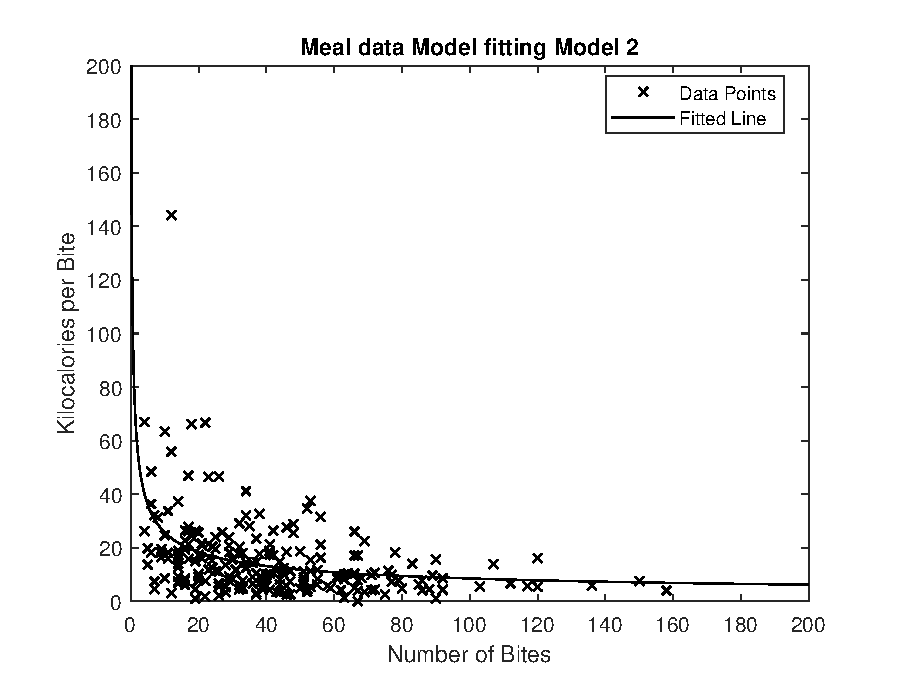
\includegraphics[scale=0.75]{fourth_result.eps}
\caption{Fitted Curve throught meal data for function $y=a(1/x^{e})+ b$ }
\label{fig:fourth_res}
\end{figure}

As compared to the first model, this model does better job at predicting the relationship between number of bites and Kilocalories per Bite.This is evident especially for the number of bites lower than 10. We can see how this model suggests the inverse relationship between number of bite and Kilocalories consumed per bite.



\afterpage{

}
\clearpage

\section{\centering Conclusion}\label{sec:conc}
In summary, we can say that normal equations provide a robust way of solving linear model fitting problems. Normal equations allow models to be accurately fitted to datasets. Moreover, this lab demonstrated how a single outlier can affect the model significantly. It is worth noting that different models can be used to fit the same data set. The model chosen greatly depends what parameters are to be observed.

\section{\centering Apendix}\label{sec:apdx}
\begin{lstlisting}[frame=single]
clear all;
clc;
% Part 1 %

c = [5,6,7,8,9];
d = [1,1,2,3,5];

A = [c' ones(5,1)];
b = [d'];
x = inv(A'*A)*A'*b
% Here first element of x is a and second element is b.%
% y = ax + b%
i = 0:0.1:10;
y = x(1)*i + x(2);
plot(c,d,"ko",i,y,"k")
xlabel("X-axis")
ylabel("Y-axis")
txt = {'First Line:','y = 1.000x-4.600'}
text(8,2,txt)
% ylim([0 6])
% legend("Data Points","Fitted Line","Location","best")
hold on
\end{lstlisting}

\begin{lstlisting}[frame=single]
% Part 2 

c1 = [5,6,7,8,8,9];
d1 = [1,1,2,3,14,5];

A1 = [c1' ones(6,1)];
b1 = [d1'];
x1 = (inv(A1'*A1)*A1')*b1

y1 = x1(1)*i + x1(2);
plot(c1(5),d1(5),"kx",i,y1,"k--") %Plotting only the outlier
ylim([0 15])
xlabel("X-axis")
ylabel("Y-axis")
legend("Data Points","First Line","Outlier","Second Line","Location","northwest")
txt = {'Second Line:','y = 1.8154x-8.6769'};
text(5,5,txt);
% hold off;
\end{lstlisting}

\begin{lstlisting}[frame=single]
% Part 3 %
data = readtable("Data.txt");
pr_data =[data.Var3 (data.Var4 ./ data.Var3)];
o = 0:1:350

plot(pr_data(1:15:end,1),pr_data(1:15:end,2),"k.")

xlabel("Number of Bites");
ylabel("Kilocalaries consumed per bite");
legend("Data Points");
title("Meal data Model fitting")
\end{lstlisting}

\begin{lstlisting}[frame=single]
%First Model%
c2 = pr_data(1:15:end,1); %Number of bites%
d2 = pr_data(1:15:end,2); %Kilocalories per bite%


A2 = [(1./(c2.^exp(1))) ones(length(c2),1)];
b2 = d2;
x2 = (inv(A2'*A2)*A2')*b2;

fn = 1./o.^exp(1);
y2 = x2(1).*fn + x2(2);
plot(c2,d2,"kx",o,y2,"k-","LineWidth",0.75)
xlim([0 200]);
ylim([0 200]);
xlabel("Number of Bites")
ylabel("Kilocalories per Bite")
legend("Data Points","Fitted Line","Location","best")
title("Meal data Model fitting Model 1")
\end{lstlisting}

\begin{lstlisting}[frame=single]
% Second model %

A3 = [(1./sqrt(c2)) ones(length(c2),1)];
b3 = d2 ; %Kilocalories per bite%;
x3 = (inv(A3'*A3)*A3')*b3;
o1 = 0:0.1:500;
fn = 1./sqrt(o1);
y3 = x3(1).*fn + x3(2);
plot(c2,d2,"kx",o1,y3,"k-","LineWidth",0.75)

xlim([0 200]);
ylim([0 200]);
xlabel("Number of Bites")
ylabel("Kilocalories per Bite")
legend("Data Points","Fitted Line","Location","best")
title("Meal data Model fitting Model 2")
\end{lstlisting}



\end{document}